
\documentclass[10pt]{beamer}
\usetheme{metropolis}

% ── Packages ──
\usepackage{amsmath,amssymb,amsthm}
\usepackage{tikz}
\usetikzlibrary{positioning,arrows.meta,fit,matrix,backgrounds,calc,shapes.geometric,decorations.pathreplacing}
\usepackage{graphicx}
\usepackage{array}
\usepackage{etoolbox}
\usepackage{cancel}

% ── Theorem environments ──
\theoremstyle{definition}
\newtheorem{defi}{Definition}[section]
\newtheorem{prop}{Proposition}[section]
\newtheorem{thm}{Theorem}[section]
\newtheorem{cor}{Corollary}[section]

% Custom theorem styles with colors
\setbeamercolor{block title}{bg=red!75!black,fg=white}
\setbeamercolor{block body}{bg=yellow!10!white}

\AtBeginEnvironment{prop}{%
  \setbeamercolor{block title}{bg=yellow!75!black,fg=black}%
  \setbeamercolor{block body}{bg=yellow!10!white}%
}
\AtEndEnvironment{prop}{%
  \setbeamercolor{block title}{bg=red!75!black,fg=white}%
}

\AtBeginEnvironment{thm}{%
  \setbeamercolor{block title}{bg=yellow!75!black,fg=black}%
  \setbeamercolor{block body}{bg=yellow!10!white}%
}
\AtEndEnvironment{thm}{%
  \setbeamercolor{block title}{bg=red!75!black,fg=white}%
}

\AtBeginEnvironment{cor}{%
  \setbeamercolor{block title}{bg=yellow!75!black,fg=black}%
  \setbeamercolor{block body}{bg=yellow!10!white}%
}
\AtEndEnvironment{cor}{%
  \setbeamercolor{block title}{bg=red!75!black,fg=white}%
}

% ── Highlighting ──
\newcommand{\x}[1]{\alert{\textbf{#1}}}

% ── Color shortcuts ──
\newcommand{\rd}[1]{{\color{red!70!black}#1}}
\newcommand{\bl}[1]{{\color{blue!70!black}#1}}
\newcommand{\gn}[1]{{\color{green!60!black}#1}}

\title{Lecture 13: Laplace Expansion}
\subtitle{MATH203 Applied Linear Algebra}
\date{}
\titlegraphic{}

\begin{document}
\maketitle


% ═══════════════════════════════════════
% §1 LAPLACE EXPANSION
% ═══════════════════════════════════════
\section{Laplace Expansion}


% ── Frame 1: Tension ──────────────────────────────────
\begin{frame}{}
\vfill
\begin{center}
{\Large Can we break a \x{big} determinant\\[6pt]
into \x{smaller} determinants?}
\end{center}
\vfill

In Lecture 12 we computed $\det$ by cross-filling.

\vfill

Today: a different decomposition --- expand \x{one column} at a time.

\vfill
\end{frame}


% ── Frame 2: Key idea ────────────────────────────────
\begin{frame}{The Key Idea: Decompose One Column}

Any column is a sum of scaled basis vectors:

\begin{columns}[T]
\begin{column}{0.45\textwidth}
\begin{center}
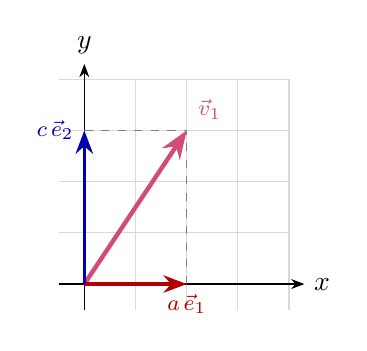
\begin{tikzpicture}[scale=0.65]
  \draw[gray!30, step=1] (-0.5,-0.5) grid (4,4);
  \draw[-{Stealth}] (-0.5,0) -- (4.3,0) node[right]{$x$};
  \draw[-{Stealth}] (0,-0.5) -- (0,4.3) node[above]{$y$};

  % Full vector
  \draw[-{Stealth}, ultra thick, purple!70] (0,0) -- (2,3)
    node[above right, font=\footnotesize]{$\vec{v}_1$};

  % Components
  \draw[-{Stealth}, very thick, red!70!black] (0,0) -- (2,0)
    node[below, font=\footnotesize]{$a\,\vec{e}_1$};
  \draw[-{Stealth}, very thick, blue!70!black] (0,0) -- (0,3)
    node[left, font=\footnotesize]{$c\,\vec{e}_2$};

  \draw[dashed, gray] (2,0) -- (2,3);
  \draw[dashed, gray] (0,3) -- (2,3);
\end{tikzpicture}
\end{center}
\end{column}
\begin{column}{0.52\textwidth}
$$
\begin{pmatrix} a \\ c \end{pmatrix}
= \rd{a}\begin{pmatrix}1\\0\end{pmatrix}
+ \bl{c}\begin{pmatrix}0\\1\end{pmatrix}
$$

\vspace{0.5cm}

By \x{multilinearity} (P1):

{\footnotesize
$\det\!\begin{pmatrix} a & b \\ c & d \end{pmatrix}
= \rd{a}\det\!\begin{pmatrix} \rd{1} & b \\ \rd{0} & d \end{pmatrix}
+ \bl{c}\det\!\begin{pmatrix} \bl{0} & b \\ \bl{1} & d \end{pmatrix}$
}
\end{column}
\end{columns}

\vfill

Each piece: column 1 replaced by $\vec{e}_i$ --- a \x{simpler} determinant!

\end{frame}


% ── Frame 3: 2×2 case ────────────────────────────────
\begin{frame}{The $2 \times 2$ Case: Nothing New}

Compute each piece:

$$
\det\begin{pmatrix} \rd{1} & b \\ \rd{0} & d \end{pmatrix}
= 1 \cdot d - 0 \cdot b = \x{d}
$$

$$
\det\begin{pmatrix} \bl{0} & b \\ \bl{1} & d \end{pmatrix}
= 0 \cdot d - 1 \cdot b = \x{-b}
$$

\vfill

Combine:
$$
\det\begin{pmatrix} a & b \\ c & d \end{pmatrix}
= \rd{a} \cdot \x{d} + \bl{c} \cdot (\x{-b})
= ad - bc \quad \checkmark
$$

\vfill

The familiar formula is just \x{Laplace expansion along column 1}!

\end{frame}


% ── Frame 4: 3×3 setup ───────────────────────────────
\begin{frame}{The $3 \times 3$ Case}

Take the matrix from Lecture 12 \;($\det = 5$ by cross-filling):

$$
A = \begin{pmatrix} 2 & 1 & 2 \\ 1 & 3 & 1 \\ 2 & 1 & 3 \end{pmatrix}
$$

\vfill

Decompose \x{column 1} into basis vectors:

$$
\begin{pmatrix} 2 \\ 1 \\ 2 \end{pmatrix}
= \rd{2}\begin{pmatrix} 1 \\ 0 \\ 0 \end{pmatrix}
+ \bl{1}\begin{pmatrix} 0 \\ 1 \\ 0 \end{pmatrix}
+ \gn{2}\begin{pmatrix} 0 \\ 0 \\ 1 \end{pmatrix}
$$

\vfill

Apply \x{multilinearity} (P1) in column 1 \ldots

\end{frame}


% ── Frame 5: Expand ──────────────────────────────────
\begin{frame}{Expanding Column 1}

P1 gives three terms --- each replaces column 1 by $\vec{e}_i$:

$$
\det(A)
= \rd{2}\det\begin{pmatrix} \rd{1} & 1 & 2 \\ \rd{0} & 3 & 1 \\ \rd{0} & 1 & 3 \end{pmatrix}
+ \bl{1}\det\begin{pmatrix} \bl{0} & 1 & 2 \\ \bl{1} & 3 & 1 \\ \bl{0} & 1 & 3 \end{pmatrix}
+ \gn{2}\det\begin{pmatrix} \gn{0} & 1 & 2 \\ \gn{0} & 3 & 1 \\ \gn{1} & 1 & 3 \end{pmatrix}
$$

\vfill

\begin{center}
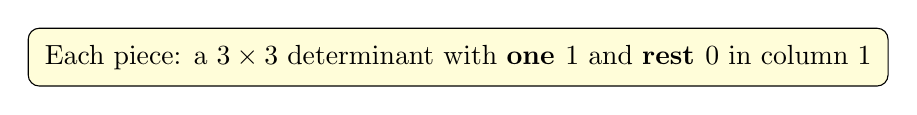
\begin{tikzpicture}
  \node[draw, rounded corners, fill=yellow!15, inner sep=6pt] {
    Each piece: a $3\times 3$ determinant with \x{one $1$} and \x{rest $0$} in column 1
  };
\end{tikzpicture}
\end{center}

\vfill

We give these pieces a name \ldots

\end{frame}


% ── Frame 6: Definition ──────────────────────────────
\begin{frame}{Algebraic Cofactor $A_{ij}$}

\begin{defi}
The \x{algebraic cofactor} $A_{ij}$ is the determinant of $A$ with \x{column $j$} replaced by $\vec{e}_i$:
$$
A_{ij} = \det\big(\vec{v}_1, \ldots, \underbrace{\vec{e}_i}_{\text{column }j}, \ldots, \vec{v}_n\big)
$$
\end{defi}

\vfill

\textbf{Recipe:} to write down $A_{ij}$, take $A$ and:
\begin{enumerate}
\item Put $\x{1}$ at position $(i,\, j)$
\item Put $\x{0}$ everywhere else in column $j$
\item Leave all other columns \x{unchanged}
\end{enumerate}

\vfill

Then compute the determinant of the result.

\end{frame}


% ── Frame 7: Compute A_11 ────────────────────────────
\begin{frame}{Computing $A_{11}$}

$$
A_{11} = \det\begin{pmatrix} \rd{1} & 1 & 2 \\ \rd{0} & 3 & 1 \\ \rd{0} & 1 & 3 \end{pmatrix}
$$

\vfill

Column 1 is $\vec{e}_1$: the $\rd{1}$ sits \x{on top}, with $\rd{0}$'s below.

This is \x{block upper triangular} (Lecture 12, \S5):

\vfill

$$
\det\begin{pmatrix} \rd{1} & 1 & 2 \\ \rd{0} & \bl{3} & \bl{1} \\ \rd{0} & \bl{1} & \bl{3} \end{pmatrix}
\quad = \quad
\rd{1} \times \det\begin{pmatrix} \bl{3} & \bl{1} \\ \bl{1} & \bl{3} \end{pmatrix}
= 9 - 1 = \x{8}
$$

\begin{center}
\textbf{Visual:} cross out the row and column where the $\rd{1}$ sits.

The remaining $\bl{2\times 2}$ block gives the answer.
\end{center}

\end{frame}


% ── Frame 8: Compute A_21, A_31 ──────────────────────
\begin{frame}{Computing $A_{21}$ and $A_{31}$}

\textbf{$A_{21}$}: column 1 is $\vec{e}_2$ --- the $\bl{1}$ is in \x{row 2}, not on top.

\quad Swap rows $1 \leftrightarrow 2$ (sign flips!), then block triangular:

$$
A_{21} = \det\begin{pmatrix} \bl{0} & 1 & 2 \\ \bl{1} & 3 & 1 \\ \bl{0} & 1 & 3 \end{pmatrix}
\;\stackrel{r_1 \leftrightarrow r_2}{=}\;
{-}\det\begin{pmatrix} 1 & 3 & 1 \\ 0 & 1 & 2 \\ 0 & 1 & 3 \end{pmatrix}
= {-}(3{-}2) = \x{-1}
$$

\vfill

\textbf{$A_{31}$}: column 1 is $\vec{e}_3$ --- the $\gn{1}$ is in \x{row 3}.

\quad Swap rows $1 \leftrightarrow 3$ (sign flips!), then block triangular:

$$
A_{31} = \det\begin{pmatrix} \gn{0} & 1 & 2 \\ \gn{0} & 3 & 1 \\ \gn{1} & 1 & 3 \end{pmatrix}
\;\stackrel{r_1 \leftrightarrow r_3}{=}\;
{-}\det\begin{pmatrix} 1 & 1 & 3 \\ 0 & 3 & 1 \\ 0 & 1 & 2 \end{pmatrix}
= {-}(6{-}1) = \x{-5}
$$

\end{frame}


% ── Frame 9: Visual pattern ──────────────────────────
\begin{frame}[fragile]{The Pattern: Cross Out and Compute}

Cross out row $i$ and column $j$ where the $1$ sits. The remaining block gives the answer (up to sign from row swaps):

\vfill

\begin{columns}[T]
\begin{column}{0.32\textwidth}
\begin{center}
{\footnotesize $A_{11}$: cross row 1, col 1}

$$\begin{pmatrix} {\color{gray}\cancel{1}} & {\color{gray}\cancel{1}} & {\color{gray}\cancel{2}} \\ {\color{gray}\cancel{0}} & \bl{3} & \bl{1} \\ {\color{gray}\cancel{0}} & \bl{1} & \bl{3} \end{pmatrix}$$

$+\det\!\left(\begin{smallmatrix}\bl{3}&\bl{1}\\\bl{1}&\bl{3}\end{smallmatrix}\right) = \x{8}$
\end{center}
\end{column}
\begin{column}{0.32\textwidth}
\begin{center}
{\footnotesize $A_{21}$: cross row 2, col 1}

$$\begin{pmatrix} {\color{gray}\cancel{0}} & \bl{1} & \bl{2} \\ {\color{gray}\cancel{1}} & {\color{gray}\cancel{3}} & {\color{gray}\cancel{1}} \\ {\color{gray}\cancel{0}} & \bl{1} & \bl{3} \end{pmatrix}$$

$-\det\!\left(\begin{smallmatrix}\bl{1}&\bl{2}\\\bl{1}&\bl{3}\end{smallmatrix}\right) = \x{-1}$
\end{center}
\end{column}
\begin{column}{0.32\textwidth}
\begin{center}
{\footnotesize $A_{31}$: cross row 3, col 1}

$$\begin{pmatrix} {\color{gray}\cancel{0}} & \bl{1} & \bl{2} \\ {\color{gray}\cancel{0}} & \bl{3} & \bl{1} \\ {\color{gray}\cancel{1}} & {\color{gray}\cancel{1}} & {\color{gray}\cancel{3}} \end{pmatrix}$$

$-\det\!\left(\begin{smallmatrix}\bl{1}&\bl{2}\\\bl{3}&\bl{1}\end{smallmatrix}\right) = \x{-5}$
\end{center}
\end{column}
\end{columns}

\end{frame}


% ── Frame 10: Verify + formula ────────────────────────
\begin{frame}{Putting It Together}

$$
\det(A) = \underbrace{\rd{2}}_{a_{11}} \cdot \underbrace{8}_{A_{11}}
\;+\; \underbrace{\bl{1}}_{a_{21}} \cdot \underbrace{({-}1)}_{A_{21}}
\;+\; \underbrace{\gn{2}}_{a_{31}} \cdot \underbrace{({-}5)}_{A_{31}}
$$

$$
= 16 - 1 - 10 = \x{5} \quad \checkmark
$$

\vfill

Matches cross-filling from Lecture 12!

\vfill

\begin{thm}[Laplace Expansion along column $j$]
$$
\boxed{\det(A) = \sum_{i=1}^{n} a_{ij} \cdot A_{ij} = a_{1j}\,A_{1j} + a_{2j}\,A_{2j} + \cdots + a_{nj}\,A_{nj}}
$$
\end{thm}

Since $\det(A^T) = \det(A)$, the same formula works for \x{rows}: fix row $i$, sum over $j$.

\end{frame}


% ── Frame 11: Strategy ───────────────────────────────
\begin{frame}{Strategy: Expand Along Zeros}

$$
\det\begin{pmatrix} 2 & 1 & 0 \\ 1 & 3 & 0 \\ 2 & 1 & 3 \end{pmatrix}
$$

\vfill
\pause

Column 3 has \x{two zeros} --- expand along it! Only one term survives:

$$
= \underbrace{0}_{a_{13}} \cdot A_{13}
+ \underbrace{0}_{a_{23}} \cdot A_{23}
+ \underbrace{\gn{3}}_{a_{33}} \cdot A_{33}
= \gn{3} \cdot A_{33}
$$

\vfill

$A_{33}$: put $1$ at $(3,3)$, zeros elsewhere in col 3. Block triangular:

$$
A_{33} = \det\begin{pmatrix} 2 & 1 & 0 \\ 1 & 3 & 0 \\ 2 & 1 & \gn{1} \end{pmatrix}
= \det\begin{pmatrix} 2 & 1 \\ 1 & 3 \end{pmatrix} = 5
$$

\vfill

$$
\det = \gn{3} \times 5 = \x{15}
$$

\end{frame}


% ── Frame 12: Practice ───────────────────────────────
\begin{frame}{Practice}

Compute by Laplace expansion (choose a good row or column!):

\vfill

\begin{enumerate}
\item $\det\begin{pmatrix} 1 & 0 & 2 \\ 0 & 3 & 0 \\ 4 & 0 & 1 \end{pmatrix} = $

\vfill

\item $\det\begin{pmatrix} 1 & 2 & 0 & 0 \\ 3 & 1 & 0 & 0 \\ 0 & 0 & 2 & 1 \\ 0 & 0 & 1 & 4 \end{pmatrix} = $

\vfill

\item For the $4\times 4$ matrix above, which is faster: Laplace or block triangular?
\end{enumerate}

\vfill

\end{frame}


% ═══════════════════════════════════════
% §2 THE ORTHOGONALITY TRICK
% ═══════════════════════════════════════
\section{The Orthogonality Trick}


% ── Frame 13: Recap ──────────────────────────────────
\begin{frame}{Recap: \rd{Column 1} Entries $\times$ \rd{Column 1} Cofactors}

$A = \begin{pmatrix} \rd{2} & 1 & 2 \\ \rd{1} & 3 & 1 \\ \rd{2} & 1 & 3 \end{pmatrix}$
\quad \rd{Column 1} entries: $\rd{2},\; \rd{1},\; \rd{2}$.

\vfill

\rd{Column 1} cofactors (replace \rd{column 1} by $\vec{e}_i$, from \S1):

{\small
$$
A_{11} = \det\begin{pmatrix} \rd{1} & 1 & 2 \\ \rd{0} & 3 & 1 \\ \rd{0} & 1 & 3 \end{pmatrix} = 8,
\quad
A_{21} = \det\begin{pmatrix} \rd{0} & 1 & 2 \\ \rd{1} & 3 & 1 \\ \rd{0} & 1 & 3 \end{pmatrix} = {-}1,
$$
$$
A_{31} = \det\begin{pmatrix} \rd{0} & 1 & 2 \\ \rd{0} & 3 & 1 \\ \rd{1} & 1 & 3 \end{pmatrix} = {-}5
$$
}

\vfill

\rd{Column 1} entries $\times$ \rd{column 1} cofactors $=$ Laplace expansion $= \det(A)$:
$$
\underbrace{\rd{2}}_{a_{11}} \cdot \underbrace{8}_{A_{11}}
\;+\; \underbrace{\rd{1}}_{a_{21}} \cdot \underbrace{({-}1)}_{A_{21}}
\;+\; \underbrace{\rd{2}}_{a_{31}} \cdot \underbrace{({-}5)}_{A_{31}}
= \x{5} = \det(A) \quad \checkmark
$$

\end{frame}


% ── Frame 14: Question ───────────────────────────────
\begin{frame}{}
\vfill
\begin{center}
{\Large What if we keep the \x{same cofactors}\\[6pt]
$A_{11} = 8, \;\; A_{21} = -1, \;\; A_{31} = -5$\\[12pt]
but multiply them by entries from\\[6pt]
a \x{different} column of $A$?}
\end{center}
\vfill
\end{frame}


% ── Frame 15: Blue column ────────────────────────────
\begin{frame}[fragile]{\bl{Column 2} Entries $\times$ Column 1 Cofactors}

Take \bl{column 2} entries from
$A = \begin{pmatrix} 2 & \bl{1} & 2 \\ 1 & \bl{3} & 1 \\ 2 & \bl{1} & 3 \end{pmatrix}$,
multiply by the \x{same} column 1 cofactors:

$$
\underbrace{\bl{1}}_{a_{12}} \cdot \underbrace{8}_{A_{11}}
\;+\; \underbrace{\bl{3}}_{a_{22}} \cdot \underbrace{({-}1)}_{A_{21}}
\;+\; \underbrace{\bl{1}}_{a_{32}} \cdot \underbrace{({-}5)}_{A_{31}}
= 8 - 3 - 5 = \x{0}
$$

\vfill

\textbf{Why?} This sum is the Laplace expansion of a \x{fake matrix} --- copy \bl{column 2} into column 1:

\begin{center}
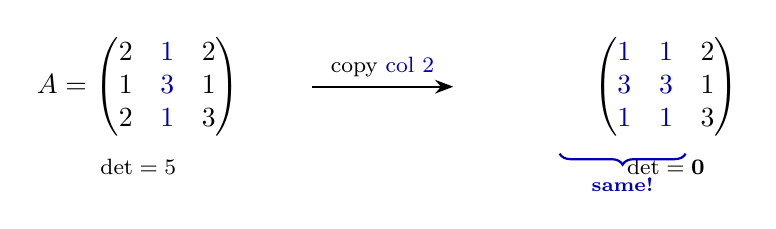
\begin{tikzpicture}
  \node (orig) at (-3.2,0) {$A = \begin{pmatrix} 2 & \bl{1} & 2 \\ 1 & \bl{3} & 1 \\ 2 & \bl{1} & 3 \end{pmatrix}$};
  \node[below=1pt of orig, font=\footnotesize] {$\det = 5$};

  \draw[-{Stealth}, thick] (-1,0) -- (0.8,0) node[midway, above, font=\footnotesize]{copy \bl{col 2}};

  \node (fake) at (3.5,0) {$\begin{pmatrix} \bl{1} & \bl{1} & 2 \\ \bl{3} & \bl{3} & 1 \\ \bl{1} & \bl{1} & 3 \end{pmatrix}$};
  \node[below=1pt of fake, font=\footnotesize] {$\det = \x{0}$};

  \draw[blue!70!black, thick, decorate,
    decoration={brace, amplitude=4pt, mirror}]
    (2.15,-0.85) -- (3.75,-0.85)
    node[midway, below=5pt, font=\scriptsize, blue!70!black]{\textbf{same!}};
\end{tikzpicture}
\end{center}

Two identical \bl{blue} columns $\Rightarrow$ P2 $\Rightarrow$ $\det = \x{0}$.

\end{frame}


% ── Frame 16: Green column ───────────────────────────
\begin{frame}[fragile]{\gn{Column 3} Entries $\times$ Column 1 Cofactors}

Take \gn{column 3} entries from
$A = \begin{pmatrix} 2 & 1 & \gn{2} \\ 1 & 3 & \gn{1} \\ 2 & 1 & \gn{3} \end{pmatrix}$,
multiply by the \x{same} column 1 cofactors:

$$
\underbrace{\gn{2}}_{a_{13}} \cdot \underbrace{8}_{A_{11}}
\;+\; \underbrace{\gn{1}}_{a_{23}} \cdot \underbrace{({-}1)}_{A_{21}}
\;+\; \underbrace{\gn{3}}_{a_{33}} \cdot \underbrace{({-}5)}_{A_{31}}
= 16 - 1 - 15 = \x{0}
$$

\vfill

\textbf{Why?} Copy \gn{column 3} into column 1:

\begin{center}
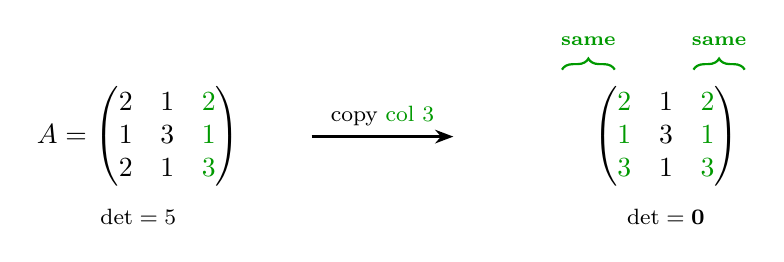
\begin{tikzpicture}
  \node (orig) at (-3.2,0) {$A = \begin{pmatrix} 2 & 1 & \gn{2} \\ 1 & 3 & \gn{1} \\ 2 & 1 & \gn{3} \end{pmatrix}$};
  \node[below=1pt of orig, font=\footnotesize] {$\det = 5$};

  \draw[-{Stealth}, thick] (-1,0) -- (0.8,0) node[midway, above, font=\footnotesize]{copy \gn{col 3}};

  \node (fake) at (3.5,0) {$\begin{pmatrix} \gn{2} & 1 & \gn{2} \\ \gn{1} & 3 & \gn{1} \\ \gn{3} & 1 & \gn{3} \end{pmatrix}$};
  \node[below=1pt of fake, font=\footnotesize] {$\det = \x{0}$};

  \draw[green!60!black, thick, decorate,
    decoration={brace, amplitude=4pt}]
    (2.18,0.85) -- (2.85,0.85)
    node[midway, above=5pt, font=\scriptsize, green!60!black]{\textbf{same}};
  \draw[green!60!black, thick, decorate,
    decoration={brace, amplitude=4pt}]
    (3.85,0.85) -- (4.5,0.85)
    node[midway, above=5pt, font=\scriptsize, green!60!black]{\textbf{same}};
\end{tikzpicture}
\end{center}

Two identical \gn{green} columns (col 1 and col 3) $\Rightarrow$ P2 $\Rightarrow$ $\det = \x{0}$.

\end{frame}


% ── Frame 17: Summary ────────────────────────────────
\begin{frame}{Summary: Right Column vs.\ Wrong Column}

All three cases with column 1 cofactors ($A_{11}{=}8,\; A_{21}{=}{-}1,\; A_{31}{=}{-}5$):

\vfill

\begin{center}
\renewcommand{\arraystretch}{1.8}
\begin{tabular}{l|c|c}
 & entries $\times$ cofactors & result \\ \hline
\rd{Col 1} entries: $\rd{2}, \rd{1}, \rd{2}$ & $= \det(A)$ by Laplace & $= \x{5}$ \\
\bl{Col 2} entries: $\bl{1}, \bl{3}, \bl{1}$ & $= \det(\text{fake: two \bl{blue} cols})$ & $= \x{0}$ \\
\gn{Col 3} entries: $\gn{2}, \gn{1}, \gn{3}$ & $= \det(\text{fake: two \gn{green} cols})$ & $= \x{0}$
\end{tabular}
\end{center}

\vfill

\x{Right} column's entries give $\det(A)$. \quad \x{Wrong} column's entries give $0$.

\vfill

\begin{center}
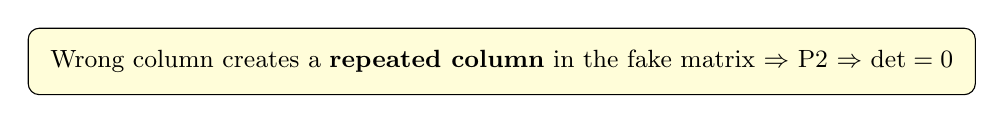
\begin{tikzpicture}
  \node[draw, rounded corners, fill=yellow!15, inner sep=8pt, font=\small] {
    Wrong column creates a \textbf{repeated column} in the fake matrix $\Rightarrow$ P2 $\Rightarrow$ $\det = 0$
  };
\end{tikzpicture}
\end{center}

\end{frame}


% ── Frame 16: Summary ────────────────────────────────
\begin{frame}{The Cofactor Orthogonality}

\begin{thm}
$$
\sum_{i=1}^{n} a_{ik} \cdot A_{ij} =
\begin{cases}
\det(A) & \text{if } k = j \quad \text{\small (right column)}\\[8pt]
0 & \text{if } k \neq j \quad \text{\small (wrong column)}
\end{cases}
$$
\end{thm}

\vfill

For our $3\times 3$ example ($\det A = 5$):

\begin{center}
\renewcommand{\arraystretch}{1.5}
{\small
\begin{tabular}{r|ccc}
& col 1 cofactors & col 2 cofactors & col 3 cofactors \\
\hline
col 1 entries & \rd{5} & $0$ & $0$ \\
col 2 entries & $0$ & \bl{5} & $0$ \\
col 3 entries & $0$ & $0$ & \gn{5}
\end{tabular}
}
\end{center}

\vfill

Diagonal $= \det(A)$, off-diagonal $= 0$. \quad This is $\det(A) \cdot I$\;!

\end{frame}


% ═══════════════════════════════════════
% §3 ADJUGATE MATRIX
% ═══════════════════════════════════════
\section{Adjugate Matrix}


% ── Frame 19: 2×2 adjugate — cofactors as determinants ──
\begin{frame}{$2\times 2$ Adjugate: Each Entry Is a Cofactor}

$A = \begin{pmatrix} 2 & 1 \\ 1 & 3 \end{pmatrix}$, \quad $\det(A) = 5$.

\vfill

Four cofactors (replace column $j$ by $\vec e_i$, take $\det$):

$$A^* = \begin{pmatrix} A_{11} & A_{21} \\ A_{12} & A_{22} \end{pmatrix}
= \begin{pmatrix}
\det\!\begin{pmatrix}\rd{1}&1\\\rd{0}&3\end{pmatrix}
& \det\!\begin{pmatrix}\rd{0}&1\\\rd{1}&3\end{pmatrix} \\[10pt]
\det\!\begin{pmatrix}2&\bl{1}\\1&\bl{0}\end{pmatrix}
& \det\!\begin{pmatrix}2&\bl{0}\\1&\bl{1}\end{pmatrix}
\end{pmatrix}
= \begin{pmatrix} 3 & -1 \\ -1 & 2 \end{pmatrix}$$

\vfill

\x{Shortcut}: swap diagonal, negate off-diagonal:\;
$\begin{pmatrix}a&b\\c&d\end{pmatrix} \;\to\; A^* = \begin{pmatrix}d&-b\\-c&a\end{pmatrix}$

\end{frame}


% ── Frame 20: A*·A setup ─────────────────────────────
\begin{frame}{Multiply: $A^* \cdot A$}

Row $i$ of $A^*$ $=$ cofactors of col $i$. \quad Column $j$ of $A$ $=$ entries of col $j$.

\vfill

$$\underbrace{\begin{pmatrix} \rd{3} & \rd{-1} \\ \bl{-1} & \bl{2} \end{pmatrix}}_{A^*}
\cdot
\underbrace{\begin{pmatrix} \rd{2} & \bl{1} \\ \rd{1} & \bl{3} \end{pmatrix}}_{A}
\;=\; ?$$

\vfill

{\small
\renewcommand{\arraystretch}{1.6}
\begin{tabular}{r|l}
entry & dot product \\ \hline
$(1,1)$: \rd{col 1} cofactors $\times$ \rd{col 1} entries
  & $\rd{3}\cdot\rd{2} + \rd{({-}1)}\cdot\rd{1}$ \\
$(1,2)$: \rd{col 1} cofactors $\times$ \bl{col 2} entries
  & $\rd{3}\cdot\bl{1} + \rd{({-}1)}\cdot\bl{3}$ \\
$(2,1)$: \bl{col 2} cofactors $\times$ \rd{col 1} entries
  & $\bl{({-}1)}\cdot\rd{2} + \bl{2}\cdot\rd{1}$ \\
$(2,2)$: \bl{col 2} cofactors $\times$ \bl{col 2} entries
  & $\bl{({-}1)}\cdot\bl{1} + \bl{2}\cdot\bl{3}$
\end{tabular}
}

\vfill

\x{Same color} $=$ matching $\;\to\;$ Laplace? \qquad \x{Mixed color} $=$ mismatch $\;\to\;$ ???

\end{frame}


% ── Frame 21: Diagonal entry (1,1) ───────────────────
\begin{frame}{Diagonal Entry $(1,1)$: Laplace Along \rd{Col 1}}

\rd{Col 1} cofactors $\times$ \rd{col 1} entries:

$$\rd{2}\cdot\underbrace{\det\!\begin{pmatrix}\rd{1}&1\\\rd{0}&3\end{pmatrix}}_{\rd{A_{11}}}
\;+\;
\rd{1}\cdot\underbrace{\det\!\begin{pmatrix}\rd{0}&1\\\rd{1}&3\end{pmatrix}}_{\rd{A_{21}}}$$

\vfill

Coefficients \rd{2}, \rd{1} go back into \rd{col 1} $\;\Longrightarrow\;$ Laplace expansion:

$$= \det\!\begin{pmatrix}\rd{2}&1\\\rd{1}&3\end{pmatrix}
= \rd{2}\cdot 3 - 1 \cdot \rd{1} = \x{5} = \det(A) \;\checkmark$$

\end{frame}


% ── Frame 22: Diagonal entry (2,2) ──────────────────
\begin{frame}{Diagonal Entry $(2,2)$: Laplace Along \bl{Col 2}}

\bl{Col 2} cofactors $\times$ \bl{col 2} entries:

$$\bl{1}\cdot\underbrace{\det\!\begin{pmatrix}2&\bl{1}\\1&\bl{0}\end{pmatrix}}_{\bl{A_{12}}}
\;+\;
\bl{3}\cdot\underbrace{\det\!\begin{pmatrix}2&\bl{0}\\1&\bl{1}\end{pmatrix}}_{\bl{A_{22}}}$$

\vfill

Coefficients \bl{1}, \bl{3} go back into \bl{col 2} $\;\Longrightarrow\;$ Laplace expansion:

$$= \det\!\begin{pmatrix}2&\bl{1}\\1&\bl{3}\end{pmatrix}
= 2\cdot\bl{3} - \bl{1}\cdot 1 = \x{5} = \det(A) \;\checkmark$$

\end{frame}


% ── Frame 23: Off-diagonal entry (1,2) ───────────────
\begin{frame}{Off-Diagonal Entry $(1,2)$: Wrong Column}

\rd{Col 1} cofactors $\times$ \bl{col 2} entries:

$$\bl{1}\cdot\underbrace{\det\!\begin{pmatrix}\rd{1}&1\\\rd{0}&3\end{pmatrix}}_{\rd{A_{11}}}
\;+\;
\bl{3}\cdot\underbrace{\det\!\begin{pmatrix}\rd{0}&1\\\rd{1}&3\end{pmatrix}}_{\rd{A_{21}}}$$

\vfill

Coefficients \bl{1}, \bl{3} go into \rd{col 1} position $\;\Longrightarrow\;$

$$= \det\!\begin{pmatrix}\bl{1}&1\\\bl{3}&3\end{pmatrix}$$

\vfill

But col 2 is also $(1,3)^T$ $\;\Longrightarrow\;$ \x{two identical columns} $\;\Longrightarrow\;$ P2 $\;\Longrightarrow\;$ $= \x{0}$

\end{frame}


% ── Frame 24: Off-diagonal entry (2,1) + conclusion ──
\begin{frame}{Off-Diagonal Entry $(2,1)$: Wrong Column Again}

\bl{Col 2} cofactors $\times$ \rd{col 1} entries:

$$\rd{2}\cdot\underbrace{\det\!\begin{pmatrix}2&\bl{1}\\1&\bl{0}\end{pmatrix}}_{\bl{A_{12}}}
\;+\;
\rd{1}\cdot\underbrace{\det\!\begin{pmatrix}2&\bl{0}\\1&\bl{1}\end{pmatrix}}_{\bl{A_{22}}}$$

\vfill

Coefficients \rd{2}, \rd{1} go into \bl{col 2} position $\;\Longrightarrow\;$

$$= \det\!\begin{pmatrix}2&\rd{2}\\1&\rd{1}\end{pmatrix}$$

\vfill

But col 1 is also $(2,1)^T$ $\;\Longrightarrow\;$ \x{two identical columns} $\;\Longrightarrow\;$ P2 $\;\Longrightarrow\;$ $= \x{0}$

\vfill

$$\therefore\;\; A^*\!\cdot A = \begin{pmatrix}\x{5}&0\\0&\x{5}\end{pmatrix} = \det(A)\cdot I_2 \;\;\checkmark$$

\end{frame}


% ── Frame 21: Cross-out shortcut ──────────────────────
\begin{frame}{Shortcut: The Cross-Out Rule}

Computing each cofactor by row-swaps is tedious. A shortcut:

\vfill

$$\boxed{A_{ij} = \underbrace{(-1)^{i+j}}_{\text{checkerboard sign}} \;\cdot\; \underbrace{\det\!\big(\text{delete row }i,\;\text{col }j\text{ from }A\big)}_{\text{minor }M_{ij}}}$$

\vfill

Sign pattern:\quad
$\begin{pmatrix} + & - & + \\ - & + & - \\ + & - & + \end{pmatrix}$

\vfill

\textbf{Verify} $A_{21}$:\; cross out row 2, col 1:

$$A_{21} = \underbrace{(-1)^{2+1}}_{-1} \cdot \underbrace{\det\!\begin{pmatrix}1&2\\1&3\end{pmatrix}}_{3-2\;=\;1} = -1 \quad\checkmark$$

\end{frame}


% ── Frame 20: Column 2 cofactors ─────────────────────
\begin{frame}{Computing \bl{Column 2} Cofactors}

$A = \begin{pmatrix} 2 & \bl{1} & 2 \\ 1 & \bl{3} & 1 \\ 2 & \bl{1} & 3 \end{pmatrix}$
\quad Cross out \bl{col 2} and the indicated row:

{\small
$$
A_{12}:\;
\underbrace{(-1)^{1+2}}_{-1} \cdot \det\!\begin{pmatrix} 1 & 1 \\ 2 & 3 \end{pmatrix}
= (-1)\cdot\underbrace{(3-2)}_{1} = \bl{{-}1}
$$

\vfill

$$
A_{22}:\;
\underbrace{(-1)^{2+2}}_{+1} \cdot \det\!\begin{pmatrix} 2 & 2 \\ 2 & 3 \end{pmatrix}
= (+1)\cdot\underbrace{(6-4)}_{2} = \bl{2}
$$

\vfill

$$
A_{32}:\;
\underbrace{(-1)^{3+2}}_{-1} \cdot \det\!\begin{pmatrix} 2 & 2 \\ 1 & 1 \end{pmatrix}
= (-1)\cdot\underbrace{(2-2)}_{0} = \bl{0}
$$
}

\end{frame}


% ── Frame 21: Column 3 cofactors ─────────────────────
\begin{frame}{Computing \gn{Column 3} Cofactors}

$A = \begin{pmatrix} 2 & 1 & \gn{2} \\ 1 & 3 & \gn{1} \\ 2 & 1 & \gn{3} \end{pmatrix}$
\quad Cross out \gn{col 3} and the indicated row:

{\small
$$
A_{13}:\;
\underbrace{(-1)^{1+3}}_{+1} \cdot \det\!\begin{pmatrix} 1 & 3 \\ 2 & 1 \end{pmatrix}
= (+1)\cdot\underbrace{(1-6)}_{-5} = \gn{{-}5}
$$

\vfill

$$
A_{23}:\;
\underbrace{(-1)^{2+3}}_{-1} \cdot \det\!\begin{pmatrix} 2 & 1 \\ 2 & 1 \end{pmatrix}
= (-1)\cdot\underbrace{(2-2)}_{0} = \gn{0}
$$

\vfill

$$
A_{33}:\;
\underbrace{(-1)^{3+3}}_{+1} \cdot \det\!\begin{pmatrix} 2 & 1 \\ 1 & 3 \end{pmatrix}
= (+1)\cdot\underbrace{(6-1)}_{5} = \gn{5}
$$
}

\end{frame}


% ── Frame 22: Adjugate definition ────────────────────
\begin{frame}{Packing Cofactors: The Adjugate $A^*$}

All 9 cofactors:\quad
{\small
\begin{tabular}{c|ccc}
 & \rd{col 1} & \bl{col 2} & \gn{col 3} \\ \hline
row 1 & $\rd{8}$ & $\bl{{-}1}$ & $\gn{{-}5}$ \\
row 2 & $\rd{{-}1}$ & $\bl{2}$ & $\gn{0}$ \\
row 3 & $\rd{{-}5}$ & $\bl{0}$ & $\gn{5}$
\end{tabular}
}

\vfill

The \x{adjugate} is the \x{transpose} of the cofactor table:
$$A^* := (\text{cofactor matrix})^T, \qquad (A^*)_{ij} = A_{ji}$$

\vfill

$$A^* = \begin{pmatrix}
\rd{8} & \rd{{-}1} & \rd{{-}5} \\
\bl{{-}1} & \bl{2} & \bl{0} \\
\gn{{-}5} & \gn{0} & \gn{5}
\end{pmatrix}
\;\longleftarrow\; \text{row } i \text{ of } A^* = \text{cofactors of col } i \text{ of } A$$

\end{frame}


% ── Frame 25: Core theorem ───────────────────────────
\begin{frame}{$3\times 3$ Verification: $A^* \cdot A = \det(A) \cdot I$}

\begin{thm}
$$\boxed{A^* \cdot A = \det(A) \cdot I_n}$$
\end{thm}

\vfill

\textbf{Row 1} of $A^*$ $= \rd{\text{col 1 cofactors}} = (\rd{8},\rd{{-}1},\rd{{-}5})$, dot with each column of $A$:

\vfill

$(\rd{8},\rd{{-}1},\rd{{-}5})\cdot(\rd{2},\rd{1},\rd{2}) = \underbrace{16-1-10}_{=\;5} = \det(A)\;\checkmark$
\quad {\footnotesize (Laplace along \rd{col 1})}

\vfill

$(\rd{8},\rd{{-}1},\rd{{-}5})\cdot(\bl{1},\bl{3},\bl{1}) = \underbrace{8-3-5}_{=\;0}\;\checkmark$
\quad {\footnotesize (\rd{col 1} cofactors $\times$ \bl{col 2} entries $\Rightarrow$ 0)}

\vfill

$(\rd{8},\rd{{-}1},\rd{{-}5})\cdot(\gn{2},\gn{1},\gn{3}) = \underbrace{16-1-15}_{=\;0}\;\checkmark$
\quad {\footnotesize (\rd{col 1} cofactors $\times$ \gn{col 3} entries $\Rightarrow$ 0)}

\vfill

{\footnotesize Rows 2, 3 of $A^*$: same pattern.\quad Result: $A^* \cdot A = 5\,I_3 \;\checkmark$}

\end{frame}


% ── Frame 24: 2×2 adjugate ──────────────────────────
\begin{frame}{$2\times 2$ Adjugate: Swap \& Negate}

$A = \begin{pmatrix}a&b\\c&d\end{pmatrix}$.\quad Using the cross-out rule:

\vfill

$$A_{11} = \underbrace{(+)}_{(-1)^{1+1}} d = d, \qquad
A_{12} = \underbrace{(-)}_{(-1)^{1+2}} c = -c$$

$$A_{21} = \underbrace{(-)}_{(-1)^{2+1}} b = -b, \qquad
A_{22} = \underbrace{(+)}_{(-1)^{2+2}} a = a$$

\vfill

Cofactor matrix $\begin{pmatrix}d&-c\\-b&a\end{pmatrix}$
\;$\xrightarrow{\;\text{transpose}\;}$\;
Adjugate $A^* = \begin{pmatrix}d&\x{-b}\\\x{-c}&a\end{pmatrix}$

\vfill

\x{Mnemonic}: \textbf{swap} diagonal entries, \textbf{negate} off-diagonal entries.

\vfill

$\begin{pmatrix}d&-b\\-c&a\end{pmatrix}\!\begin{pmatrix}a&b\\c&d\end{pmatrix} = \begin{pmatrix}ad-bc&0\\0&ad-bc\end{pmatrix} = (ad-bc)\,I_2 \;\checkmark$

\end{frame}


% ═══════════════════════════════════════
% §4 INVERSE VIA ADJUGATE
% ═══════════════════════════════════════
\section{Inverse via Adjugate}


% ── Frame 25: Inverse formula ────────────────────────
\begin{frame}{The Inverse Formula}

From $A^* \cdot A = \det(A) \cdot I$, divide both sides by $\det(A)$:

\vfill

\begin{thm}
If $\det(A) \neq 0$:
$$\boxed{A^{-1} = \frac{1}{\det(A)}\; A^*}$$
\end{thm}

\vfill

\textbf{Our example}: $\det(A) = 5 \neq 0$, so

$$A^{-1} = \frac{1}{5}\begin{pmatrix} 8 & -1 & -5 \\ -1 & 2 & 0 \\ -5 & 0 & 5\end{pmatrix}$$

\end{frame}


% ── Frame 26: Invertibility equivalence ──────────────
\begin{frame}{When Is a Matrix Invertible?}

\begin{thm}
$$\boxed{A \text{ is invertible} \;\Longleftrightarrow\; \det(A) \neq 0}$$
\end{thm}

\vfill

\textbf{Proof} ($\Leftarrow$): \; If $\det(A)\neq 0$, we just built the inverse:
$$A^{-1} = \frac{1}{\det(A)}\, A^*$$

\vfill

\textbf{Proof} ($\Rightarrow$): \; If $A$ is invertible, then $AA^{-1} = I$, so
$$\det(A)\,\det(A^{-1}) = \det(I) = 1 \;\;\Longrightarrow\;\; \det(A) \neq 0$$

\vfill

\textbf{Contrapositive}: \; $\det(A) = 0 \;\Longrightarrow\;$ $A$ is \x{not invertible} (columns are linearly dependent)

\end{frame}


% ── Frame 27: 2×2 inverse ───────────────────────────
\begin{frame}{$2\times 2$ Inverse Formula}

\begin{thm}
$$\begin{pmatrix}a&b\\c&d\end{pmatrix}^{-1} = \frac{1}{ad-bc}\begin{pmatrix}d&-b\\-c&a\end{pmatrix}$$
\end{thm}

\vfill

\textbf{Example}: $\begin{pmatrix}2&1\\1&3\end{pmatrix}^{-1}$

$$= \frac{1}{\underbrace{2\cdot3 - 1\cdot1}_{5}}\begin{pmatrix}3&-1\\-1&2\end{pmatrix} = \begin{pmatrix}\frac{3}{5}&-\frac{1}{5}\\[4pt]-\frac{1}{5}&\frac{2}{5}\end{pmatrix}$$

\vfill

Verify: $\begin{pmatrix}2&1\\1&3\end{pmatrix}\begin{pmatrix}3/5&-1/5\\-1/5&2/5\end{pmatrix} = \begin{pmatrix}1&0\\0&1\end{pmatrix}\;\checkmark$

\end{frame}


% ═══════════════════════════════════════
% §5 CRAMER'S RULE
% ═══════════════════════════════════════
\section{Cramer's Rule}


% ── Frame 27: Derive Cramer from 2×2 ────────────────
\begin{frame}{From Adjugate to Cramer}

For $\begin{pmatrix}a&b\\c&d\end{pmatrix}\begin{pmatrix}x\\y\end{pmatrix} = \begin{pmatrix}p\\q\end{pmatrix}$,
the inverse formula gives:

$$x = \frac{dp - bq}{ad - bc}, \qquad y = \frac{aq - cp}{ad - bc}$$

\vfill

Look at the numerator of $x$:

$$\underbrace{dp - bq}_{\text{numerator}} = \det\begin{pmatrix}\rd{p}&b\\\rd{q}&d\end{pmatrix} \quad\longleftarrow\; A \text{ with \rd{col 1} replaced by } \begin{pmatrix}p\\q\end{pmatrix}$$

\vfill

Look at the numerator of $y$:

$$\underbrace{aq - cp}_{\text{numerator}} = \det\begin{pmatrix}a&\rd{p}\\c&\rd{q}\end{pmatrix} \quad\longleftarrow\; A \text{ with \rd{col 2} replaced by } \begin{pmatrix}p\\q\end{pmatrix}$$

\vfill

\x{Pattern}: $x_i = \dfrac{\det(A_i)}{\det(A)}$ where $A_i$ = replace column $i$ by $b$!

\end{frame}


% ── Frame 28: Cramer's formula ───────────────────────
\begin{frame}{Cramer's Rule}

\begin{thm}[Cramer's Rule]
If $\det(A) \neq 0$ and $Ax = b$, then
$$\boxed{x_i = \frac{\det(A_i)}{\det(A)}}$$
where $A_i$ = $A$ with \x{column $i$ replaced by $b$}.
\end{thm}

\vfill

\textbf{Visually} for $3\times 3$: which column gets replaced?

{\small
$$A_1 = \begin{pmatrix}\rd{b_1}&a_{12}&a_{13}\\\rd{b_2}&a_{22}&a_{23}\\\rd{b_3}&a_{32}&a_{33}\end{pmatrix},\quad
A_2 = \begin{pmatrix}a_{11}&\rd{b_1}&a_{13}\\a_{21}&\rd{b_2}&a_{23}\\a_{31}&\rd{b_3}&a_{33}\end{pmatrix},\quad
A_3 = \begin{pmatrix}a_{11}&a_{12}&\rd{b_1}\\a_{21}&a_{22}&\rd{b_2}\\a_{31}&a_{32}&\rd{b_3}\end{pmatrix}$$
}

\vfill

{\footnotesize Why? Cofactors of col $i$ depend only on other columns --- same in $A$ and $A_i$.\\
So $\sum_k A_{ki} b_k$ = Laplace expansion of $\det(A_i)$ along col $i$.}

\end{frame}


% ── Frame 29: 2×2 Cramer example ────────────────────
\begin{frame}{Example: Cramer's Rule}

$\begin{pmatrix}2&1\\1&3\end{pmatrix}\begin{pmatrix}x\\y\end{pmatrix} = \begin{pmatrix}5\\5\end{pmatrix}$, \quad $\det(A) = \underbrace{6-1}_{5}$.

\vfill

$$x = \frac{\det\begin{pmatrix}\rd{5}&1\\\rd{5}&3\end{pmatrix}}{\det(A)}
= \frac{\overbrace{15-5}^{10}}{5} = \x{2}$$

\vfill

$$y = \frac{\det\begin{pmatrix}2&\rd{5}\\1&\rd{5}\end{pmatrix}}{\det(A)}
= \frac{\overbrace{10-5}^{5}}{5} = \x{1}$$

\vfill

Check: $\begin{pmatrix}2&1\\1&3\end{pmatrix}\begin{pmatrix}2\\1\end{pmatrix} = \begin{pmatrix}5\\5\end{pmatrix}\;\checkmark$

\end{frame}


% ── Frame 30: Practice ──────────────────────────────
\begin{frame}{Practice}

\begin{enumerate}
\item Use Cramer's Rule to solve:

$$\begin{pmatrix}2&1&2\\1&3&1\\2&1&3\end{pmatrix}\begin{pmatrix}x_1\\x_2\\x_3\end{pmatrix} = \begin{pmatrix}7\\6\\8\end{pmatrix}$$

{\footnotesize Hint: $\det(A) = 5$. Use $x_i = \frac{1}{\det A}\,(\text{row }i\text{ of }A^*)\cdot b$ --- you know all the cofactors!}

\vfill

\item Find $\begin{pmatrix}2&3\\1&2\end{pmatrix}^{-1}$ using the adjugate formula.

\vfill

\item True or False: if $\det(A) = 0$, then $Ax = b$ has no solution.
\end{enumerate}

\end{frame}


% ── Frame 31: Summary ───────────────────────────────
\begin{frame}{Summary}

\begin{enumerate}
\item \textbf{Cross-out rule}: $A_{ij} = (-1)^{i+j} M_{ij}$

\item \textbf{Adjugate}: $A^* = (\text{cofactor matrix})^T$, \quad $A \cdot A^* = \det(A) \cdot I$

\item \textbf{Inverse}: $A^{-1} = \dfrac{1}{\det A}\, A^*$ \quad (when $\det A \neq 0$)

\item \textbf{Cramer}: $x_i = \dfrac{\det(A_i)}{\det(A)}$
\end{enumerate}

\vfill

All from \x{two properties}: multilinearity (P1) + alternating (P2)!

\end{frame}


\end{document}
